\documentclass[12pt, a4paper]{article}
%\usepackage{a4wide}%
\usepackage{geometry}
\usepackage{ucs}
\usepackage{caption}
\usepackage{graphicx}
\usepackage[T1]{fontenc}
\usepackage{selinput} 
\usepackage[german]{babel}
\usepackage{float}
\usepackage{listings}
\usepackage{lastpage}
\usepackage{amsmath}

\geometry{,
  margin=2.54cm
}

\SelectInputMappings{ 
  adieresis={ä}, 
  germandbls={ß}, 
  Euro={€} 
}

\pagenumbering{arabic}
\usepackage{color}
\definecolor{softGray}{RGB}{160,160,160}
\definecolor{softOrange}{RGB}{255,140,15}
\definecolor{darkGreen}{RGB}{35,110,37}
\definecolor{darkRed}{RGB}{136,19,80}
\definecolor{stringColor}{RGB}{118,15,21}
\definecolor{identColor}{RGB}{0,51,105}
\definecolor{typeColor}{RGB}{0,69,176}
\definecolor{keywordColor}{RGB}{0,69,176}
\definecolor{gray}{RGB}{160,160,160}
\definecolor{lightBlue}{RGB}{44,152,242}
\definecolor{commentColor}{RGB}{135,135,135}
\definecolor{stringColor}{RGB}{221,36,0}
\definecolor{identifierColor}{RGB}{63,110,125}
\definecolor{bluekeywords}{rgb}{0.13,0.13,1}
\definecolor{greencomments}{rgb}{0,0.5,0}
\definecolor{bluestrings}{rgb}{0.13,0.5,0.5}

\setlength{\parskip}{\baselineskip}
\setlength{\parindent}{0pt} 

\makeatletter
\title{Semesterassignment} \let\Title\@title
\author{Rotaru Daniel} \let\Author\@author
\makeatother
\usepackage{fancyhdr}
\pagestyle{fancy}
\cfoot{\thepage\ of \pageref{LastPage} }

\begin{document}
\lstset{language=csh,
				extendedchars=\true,
				inputencoding=utf8,
				breakatwhitespace=false,
        breaklines=true,
        stepnumber=2,
        basicstyle=\ttfamily\scriptsize,
        columns=fullflexible,
        showspaces=false,
        showstringspaces=false,
        keywordstyle=\bf\color{bluekeywords},
        commentstyle=\color{greencomments},
        stringstyle=\color{bluestrings},
        showtabs=false,
        tabsize=2
        }


\section{Ultimate Festival Organizer (UFO)}

\subsection{Datenmodell}

\begin{figure}[h] 	
	\centering
		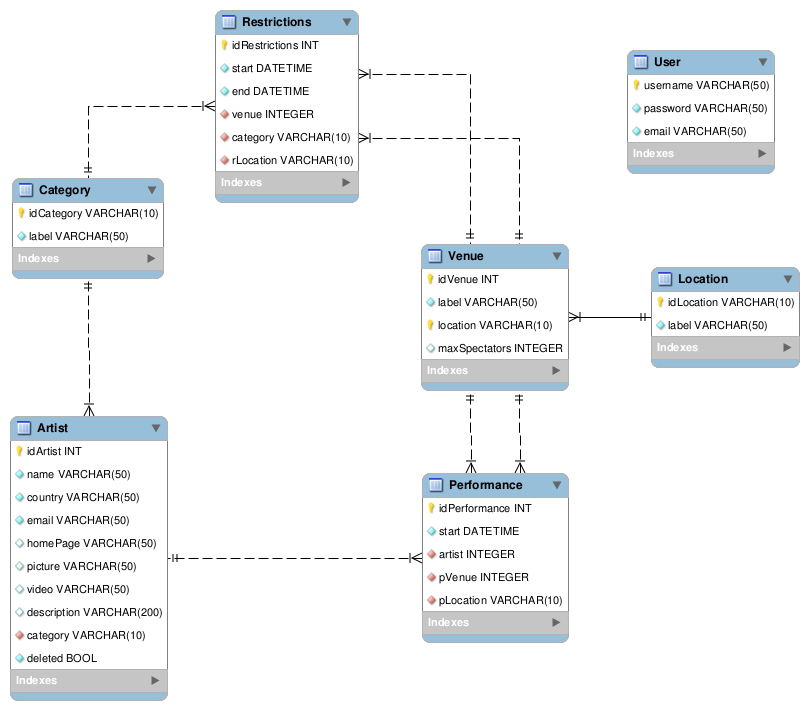
\includegraphics[width=0.7\textwidth]{DbDiagramm.png}
	\caption{OR-Diagramm}
\end{figure}

Das Datenmodell enthält zusätzlich zu den vorgegebenen Entitäten zwei weitere Entitäten: \textit{Location}-Entität und \textit{Restrictions}-Entität. Die \textit{Location}-Entität enthält als Primärschlüssel eine kurze Bezeichnung einer bestimmter Ort und der vollständige Name des Ortes, z.B. H - Hauptplatz, L - Landstraße. Der Primärschlüssel der \textit{Location}-Entität wird als Fremdschlüssel und gleichzeitig Primärschlüssel in der Spielstätte-Entität verwendet. Die Spielstätte-Entität besitzt einen zusammengesetzten Primärschlüssel aus zwei Attributen: \textit{idVenue} und der Fremdschlüssel \textit{location}. Das Attribut \textit{idVenue} wird nicht automatisch inkrementiert, sondern wird von Programm bestimmt, indem man der Anzahl an aktuell existierende Spielstätte für ein bestimmtes Ort um eins inkrementiert und als nächstes \textit{idVenue} speichert. Dadurch schafft man, dass die \textit{idVenue} für ein bestimmtes Ort, z.B. Hauptplatz, nicht größer wird als der Tatsächlichen Anzahl an Spielstätten für diesen Ort.

Die Entität \textit{Restrictions} kann benutzt werden, um bestimmte Darbietungskategorien einschränken zu können. Zum Beispiel kann eine mögliche Kategorie für Kinder so eingeschränkt, dass die Aufführungen für Kinder nur während einer bestimmten Zeitspanne vorgetragen werden können. Auch Feueraufführungen sollen nur zwischen 21 und 23 Uhr stattfinden, da zu diesem Zeitpunkt das Tageslicht nicht mehr so stakt ist. 

Die Entität \textit{Artist} Besitz ein Attribut der Typ Bool \textit{deleted}, der gesetzt wird, falls ein Künstler gelöscht werden soll. Damit wird der Künstler als gelöscht markiert, wird aber nicht aus der Datenbank gelöscht.

\subsection{Datenzugriffsschicht}

Um eine möglich gute Abstraktion zu erreichen wurde eine generische \textit{IDao}-Interface implementiert. Jede \textit{Dao} muss diese Interface implementieren.

\begin{figure}[h] 	
	\centering
		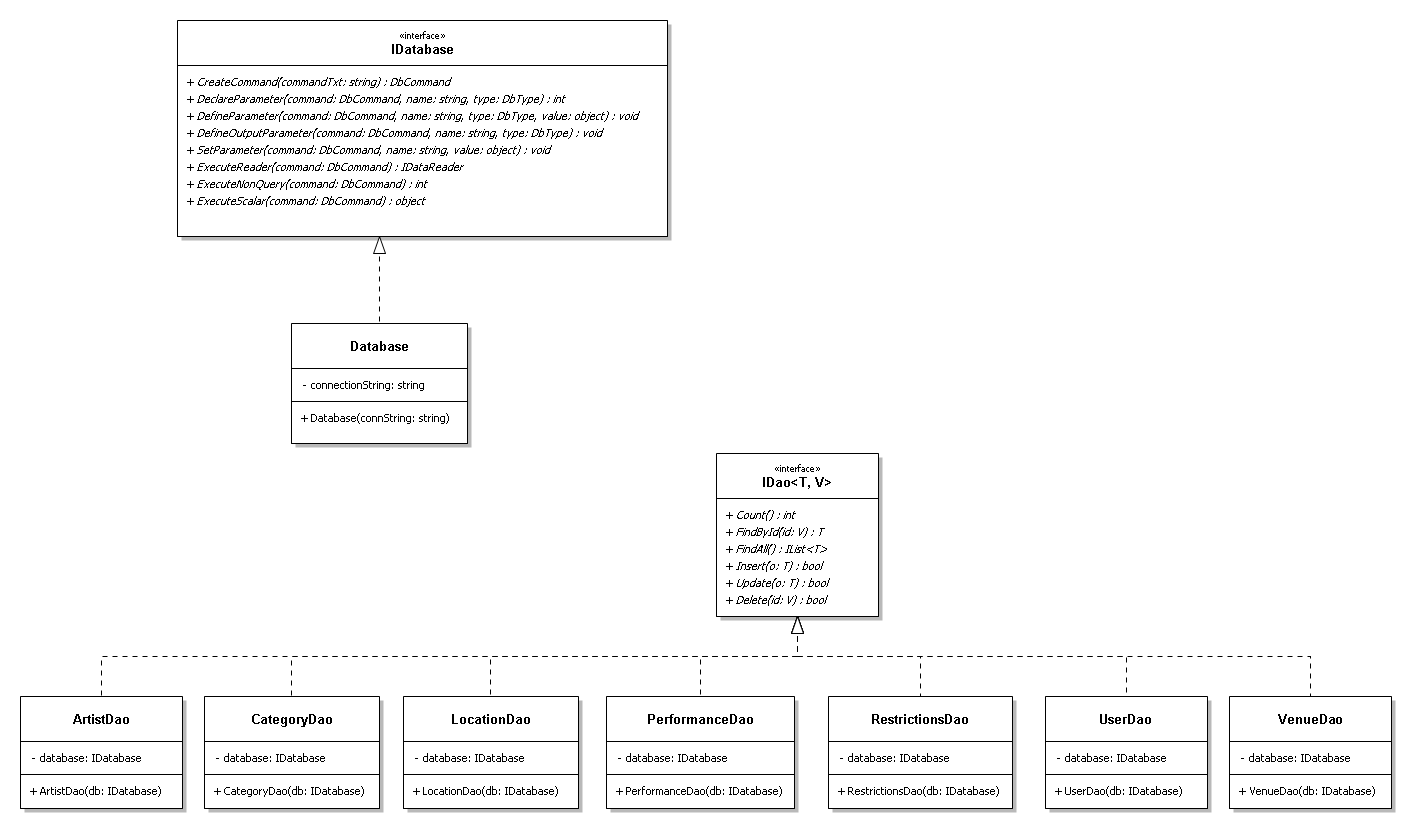
\includegraphics[width=0.7\textwidth]{Dao.png}
	\caption{Data Access}
\end{figure}

Um die Daten besser zwischen unterschiedlichen Schichten zu transportieren, wurde für jede Entität eine eigene \textit{Domain}-Klasse implementiert.

\begin{figure}[h] 	
	\centering
		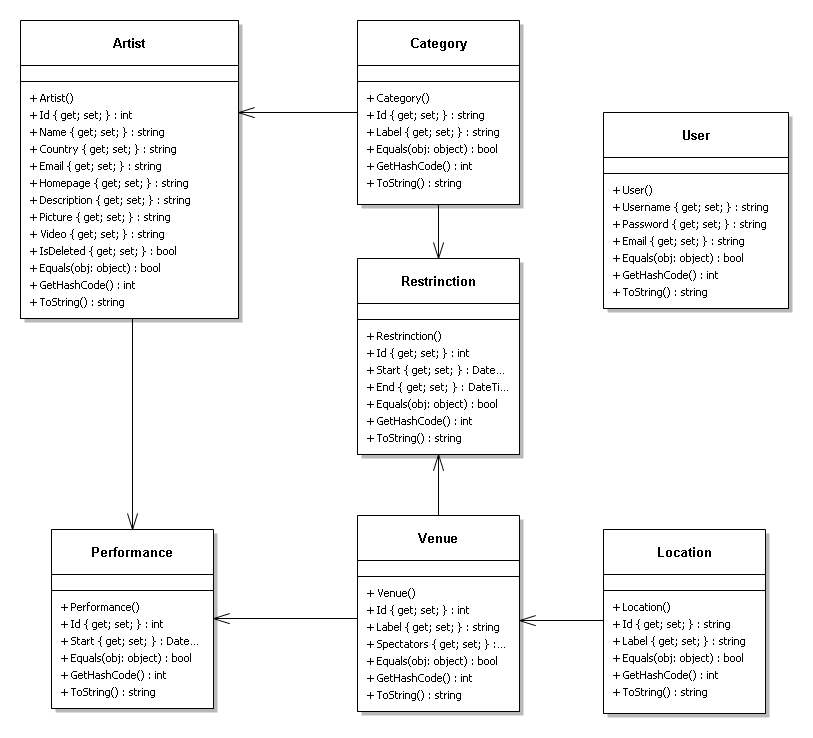
\includegraphics[width=0.6\textwidth]{DomainClasses.png}
	\caption{Domain Classes}
\end{figure}

\subsection{Unit-Tests}

\begin{figure}[h] 	
	\centering
		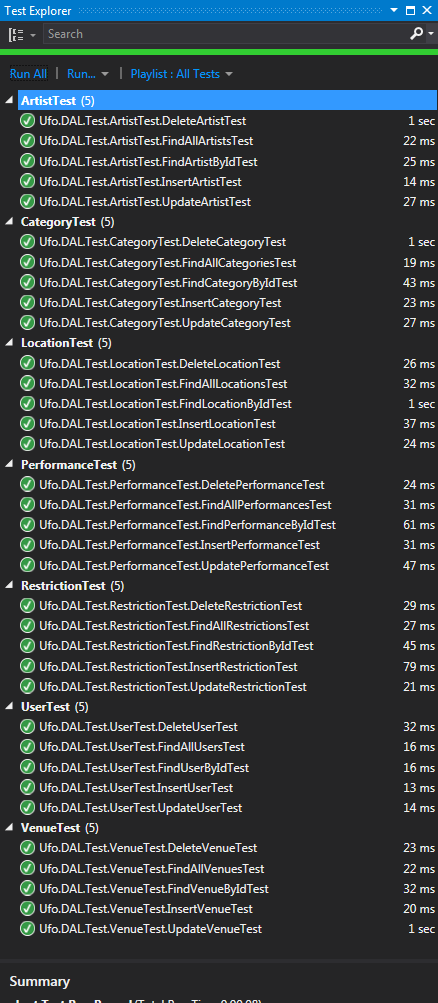
\includegraphics[width=0.5\textwidth]{UnitTests.png}
	\caption{Ergebnis Unit-Tests}
\end{figure}


Für jede implementierte DAO-Methode wurde jeweils ein Unit-Test implementiert. Dafür wurde eine eigene Testdatenbank erstellt. Als Testumgebung wurde XUnit-Framework verwendet. Diesen \textit{Framework} bietet ein \textit{AutoRollback}-Attribut, der von Entwickler implementiert werden muss. Diesen Attribut verwendet Datenbanktransaktionen um die Unit-Test Daten nicht in die Datenbank zu speichern. Damit gibt es keine Abhängigkeit zwischen einzelnen Unit-Tests und jeden Unit-Test ist atomar.

\clearpage

\lstinputlisting{../Ufo/Ufo.DAL.Test/AutoRollbackAttribute.cs}


\end{document}